\documentclass{beamer}
\usepackage[utf8]{inputenc}
\usepackage[english,russian]{babel}
\usepackage{graphicx}
\usepackage{sidecap}

%beamer  theme's used to be here :)
\usetheme{mipt_beamer}

\title{Применение взаимодействующих нейронных сетей в криптографии}
\author{Ходаков Дмитрий.}
\date{March 14, 2014} %\today

\begin{document}
\frame{\titlepage}
\frame{\tableofcontents}

\section{Постановка задачи}

\subsection{Передача ключей}

\begin{frame}
\frametitle{Передача ключей}
\begin{itemize}
\item Безопасная замена алгоритма Диффи-Хеллмана
\item Основана на синхронизации двух нейросетей
\item Они называются древовидных машин четности (TPM, tree parity machines)
\end{itemize} 
\end{frame}

\subsection{Tree Parity Machines}

\begin{frame}
\frametitle{Tree Parity Machines}
\begin{itemize}
\item Многоуровневая нейронная сети прямого распространения
\item Входные нейроны принимают значения \(x_{i} \in \left\{ -1,+1 \right\}\)
\item Веса принимают значения \(w_{i} \in \left\{-L,...,0,...,+L \right\}\)
\item Значения скрытого нейрона \(\sigma_i=sgn(\sum_{j=1}^{N}w_{ij}x_{ij})\)
\item Значения выходного нейрона \(\tau=\prod_{i=1}^{K}\sigma_i\)
\end{itemize} 
\begin{center}
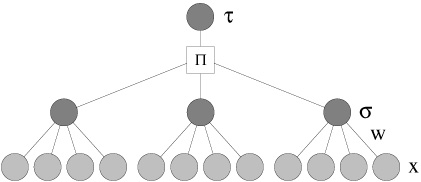
\includegraphics[width=10cm, height=5cm]{../../pics/tpmv2.jpg}
\end{center}
\end{frame}


\begin{frame}
\frametitle{Tree Parity Machines - алгоритм}
У каждого абонента (А или Б) есть своя TPM. 
Синхронизация:
\begin{itemize}

\item Задаём случайные значения весовых коэффициентов
\item Выполняем следующие шаги, пока не наступит синхронизация
\item Генерируем случайный входной вектор X
\item Вычисляем значения скрытых нейронов
\item Вычисляем значение выходного нейрона
\item Сравниваем выходы двух TPM:
\item Выходы разные: переход к п.2.1
\item Выходы одинаковые: применяем выбранное правило к весовым коэффициентам
\end{itemize} 
\end{frame}

\begin{frame}
\frametitle{Tree Parity Machines - алгоритм}
Для обновления весовых коэффициентов могут использоваться следующие правила:


\begin{itemize}

\item Правило Хебба: \(w_i^+=w_i+\sigma_ix_i\Theta(\sigma_i\tau)\Theta(\tau^A\tau^B)\)

\item Обратное правило Хебба: \(w_i^+=w_i-\sigma_ix_i\Theta(\sigma_i\tau)\Theta(\tau^A\tau^B)\)

\item Случайное блуждание: \(w_i^+=w_i+x_i\Theta(\sigma_i\tau)\Theta(\tau^A\tau^B)\)

\end{itemize}
\end{frame}

\subsection{Устойчивость к атакам}
\begin{frame}
\frametitle{Устойчивость к атакам}
\begin{itemize}
\item Перебор:  \((2L+1)^{KN}\) вариантов - неэффективно
\item Синхронное обучение:  Длительная синхронизация (10-100 и более раз) - неэффективно
\item Другие атаки: геометрическая, вероятностный анализ, генетические алгоритмы
\end{itemize}
\end{frame}


\section{Результаты}

\subsection{Зависимость скорости сходимости от N}
\begin{frame}
\frametitle{Зависимость скорости сходимости от N}
Правило Хебба, L=3, K=3
\begin{center}
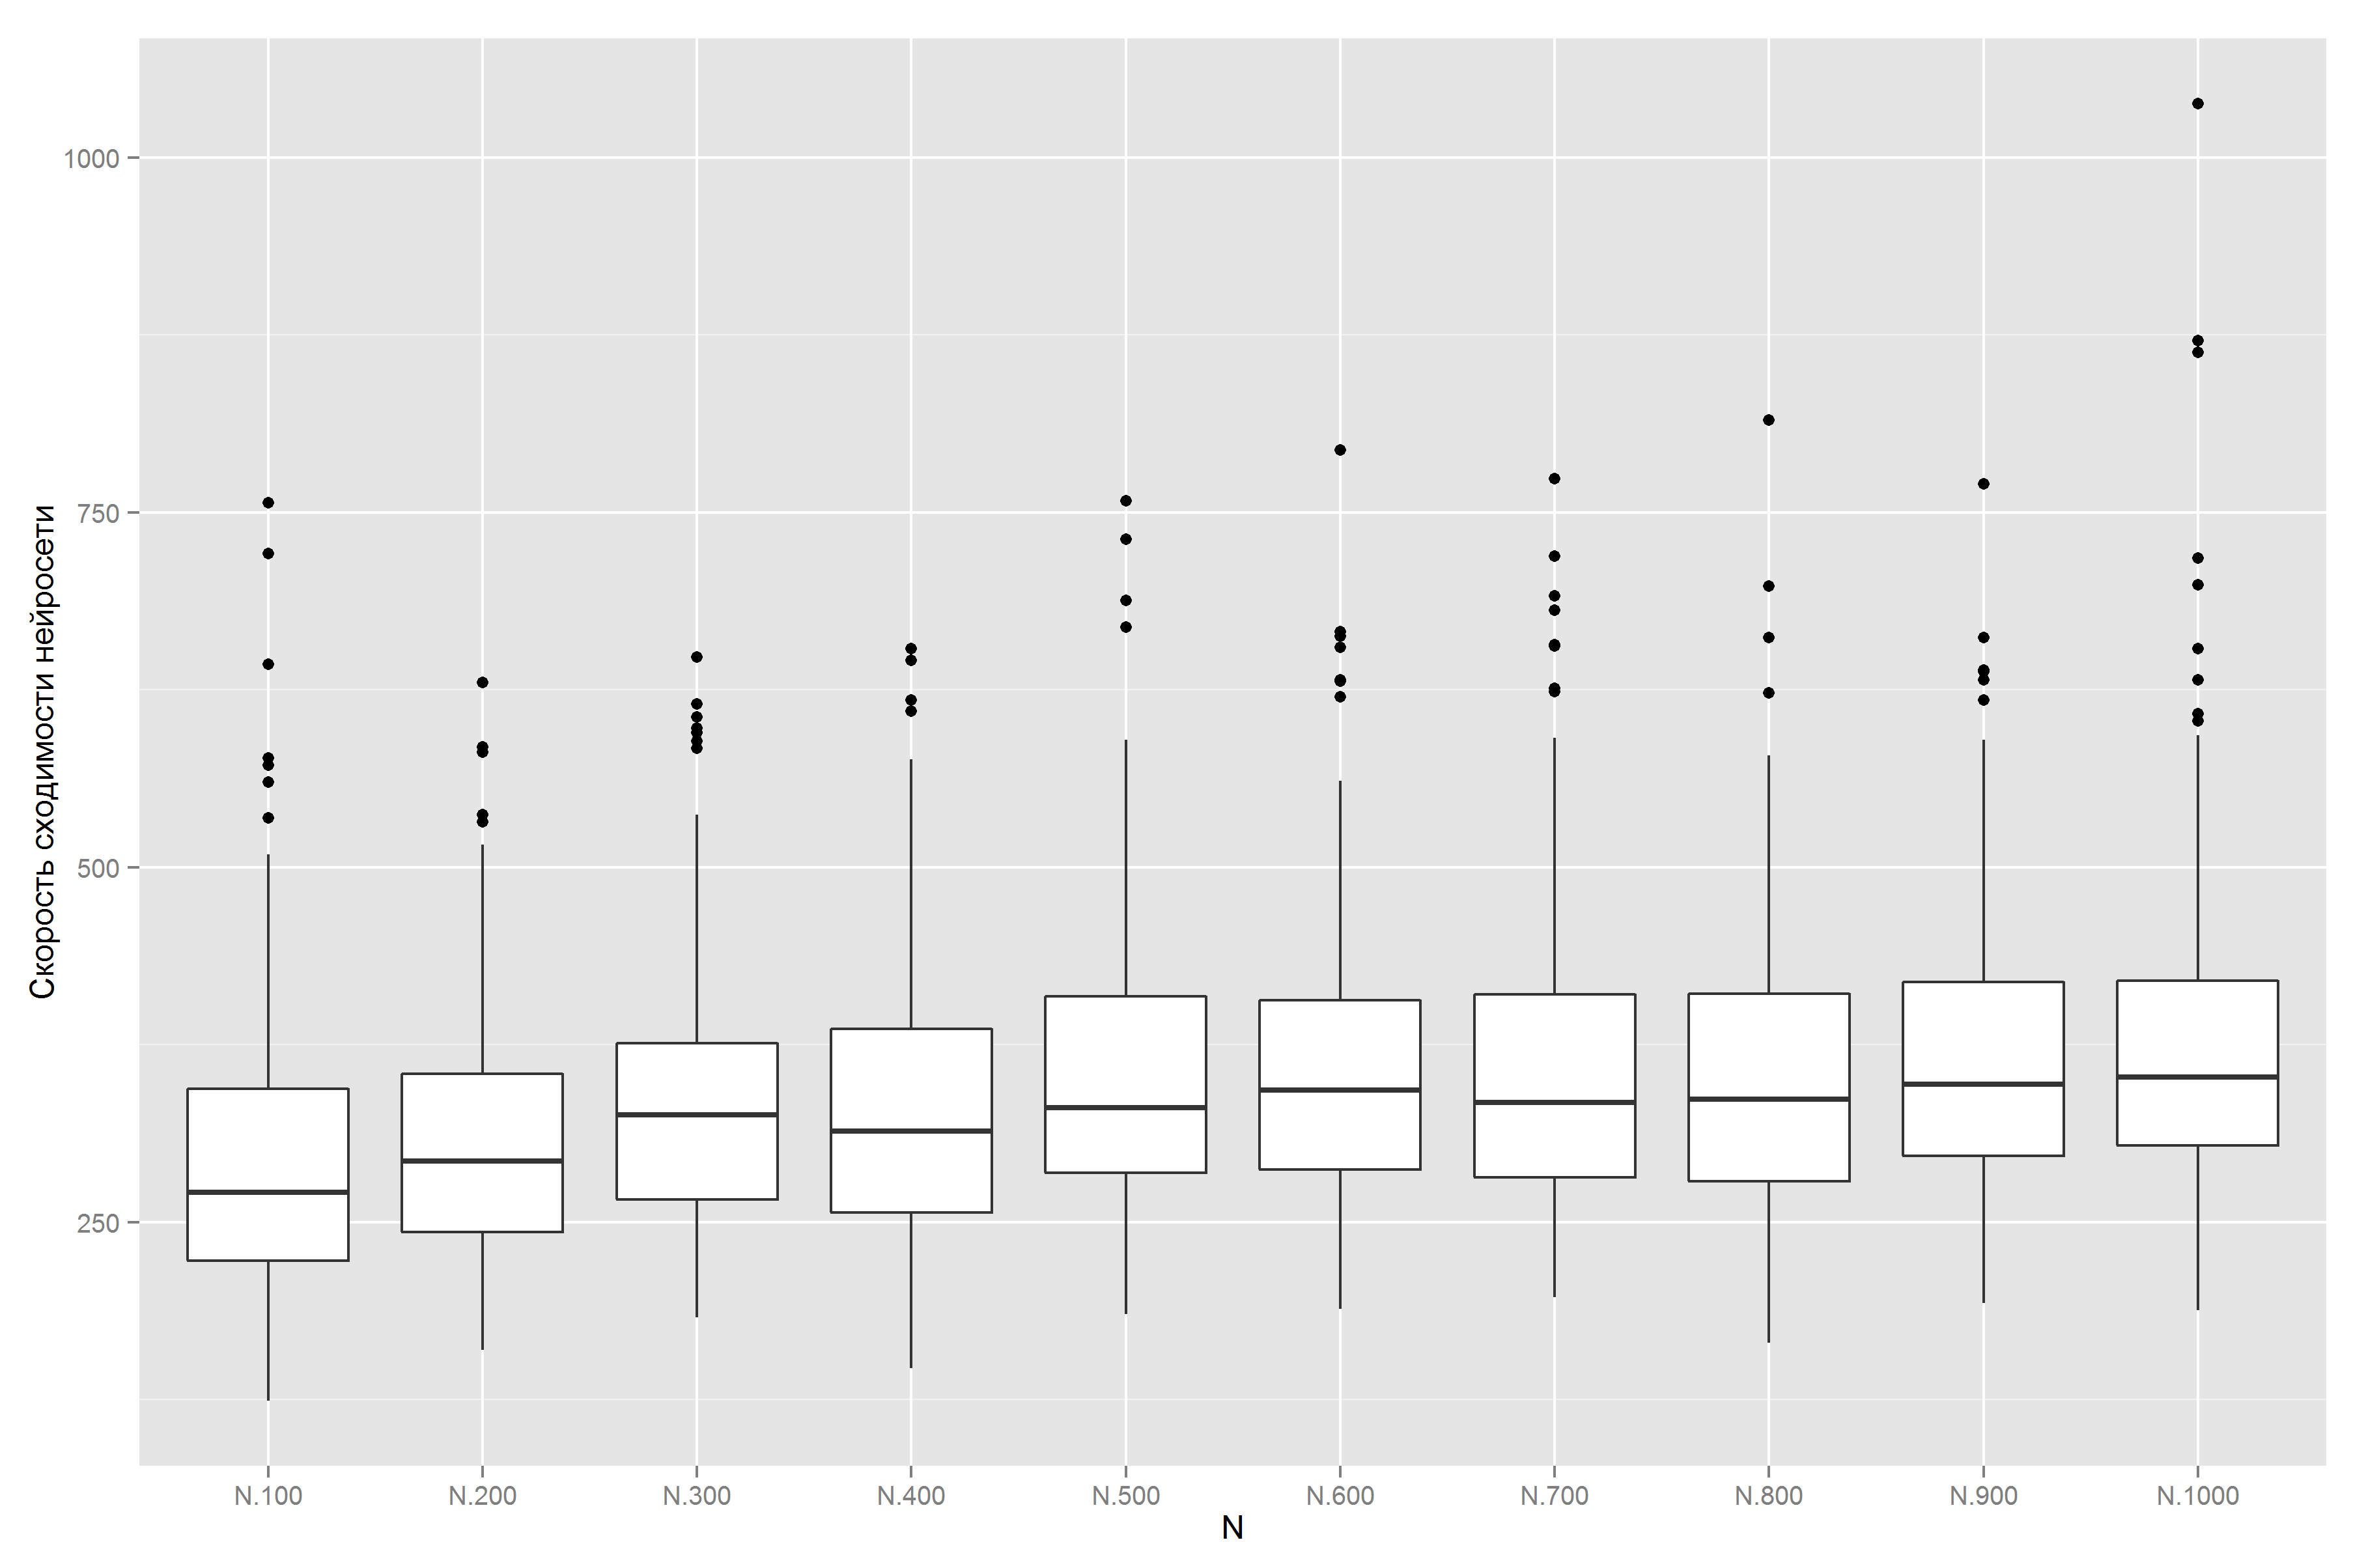
\includegraphics[width=10cm, height=7cm]{../../plots/l3pn3N_vs_tsync_100.png}

\end{center}
\end{frame}

\begin{frame}
\frametitle{Зависимость скорость схождения сети от L}
Правило Хебба, N=100, K=3
\begin{center}
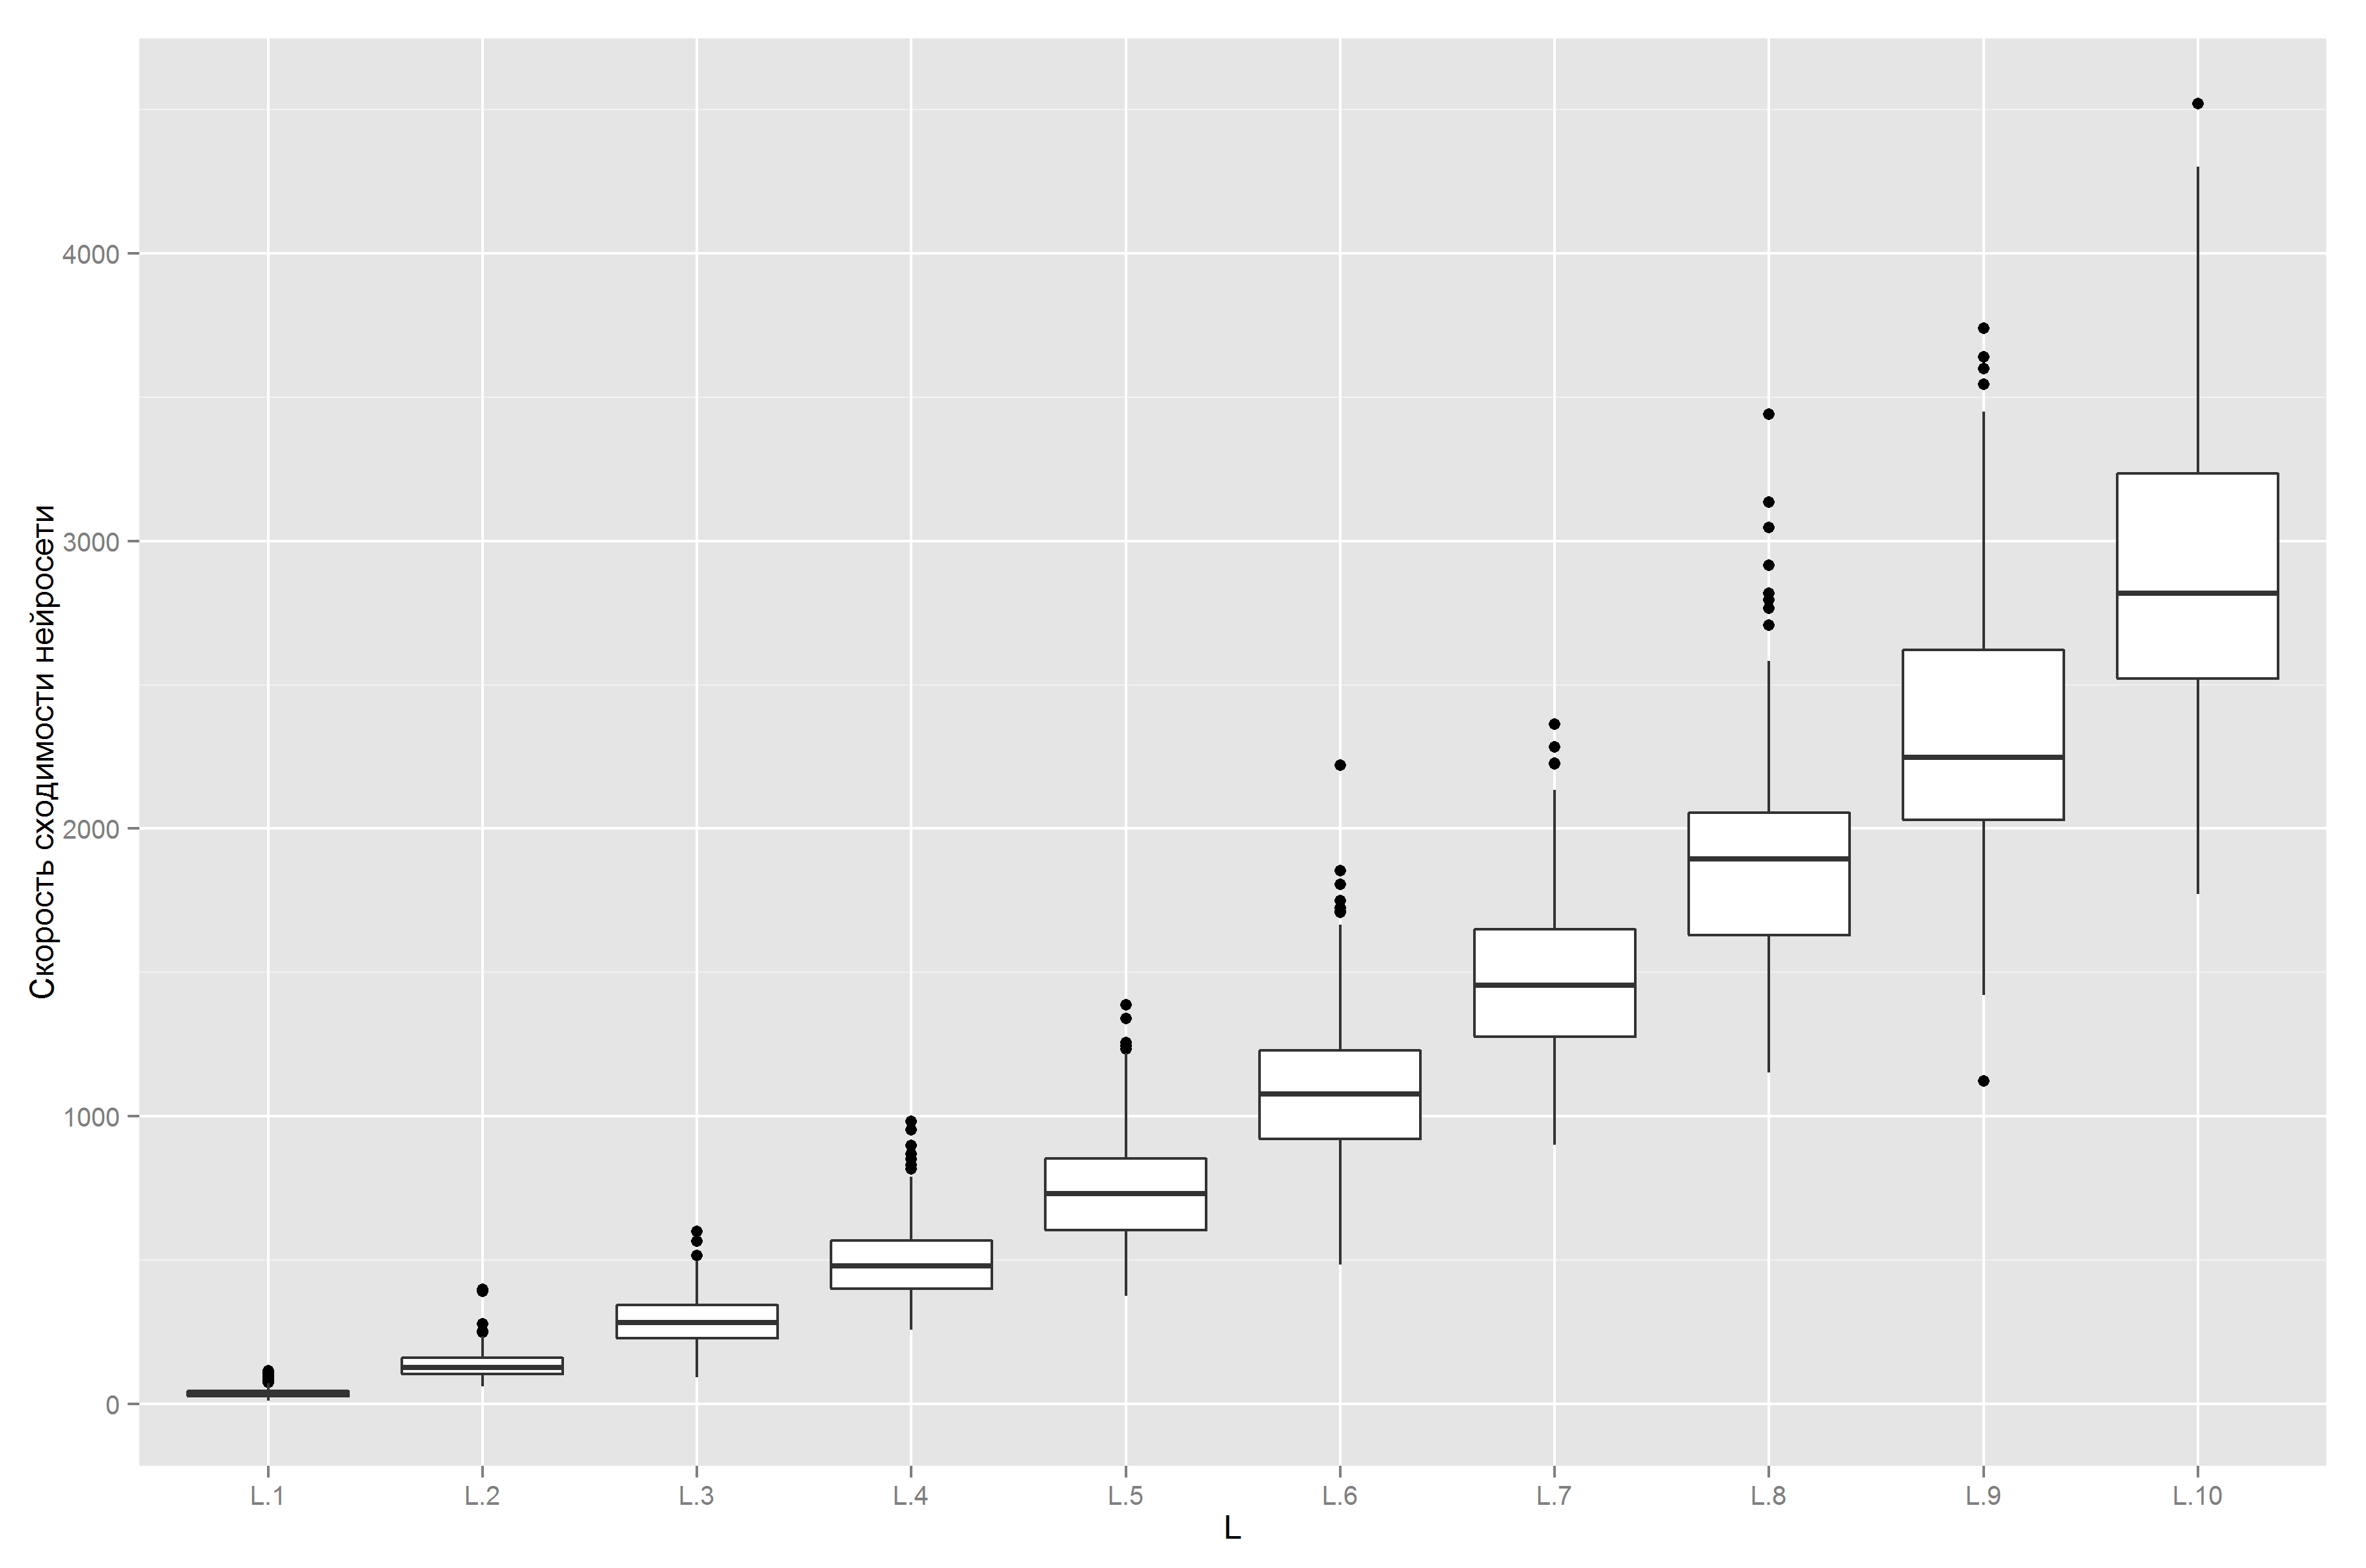
\includegraphics[width=10cm, height=7cm]{../../plots/n100pn3LvsTsync.png}

\end{center}
\end{frame}

\begin{frame}
\frametitle{От кол-ва связей на 1м слое}
Правило Хебба, N=100, L=3
\begin{center}
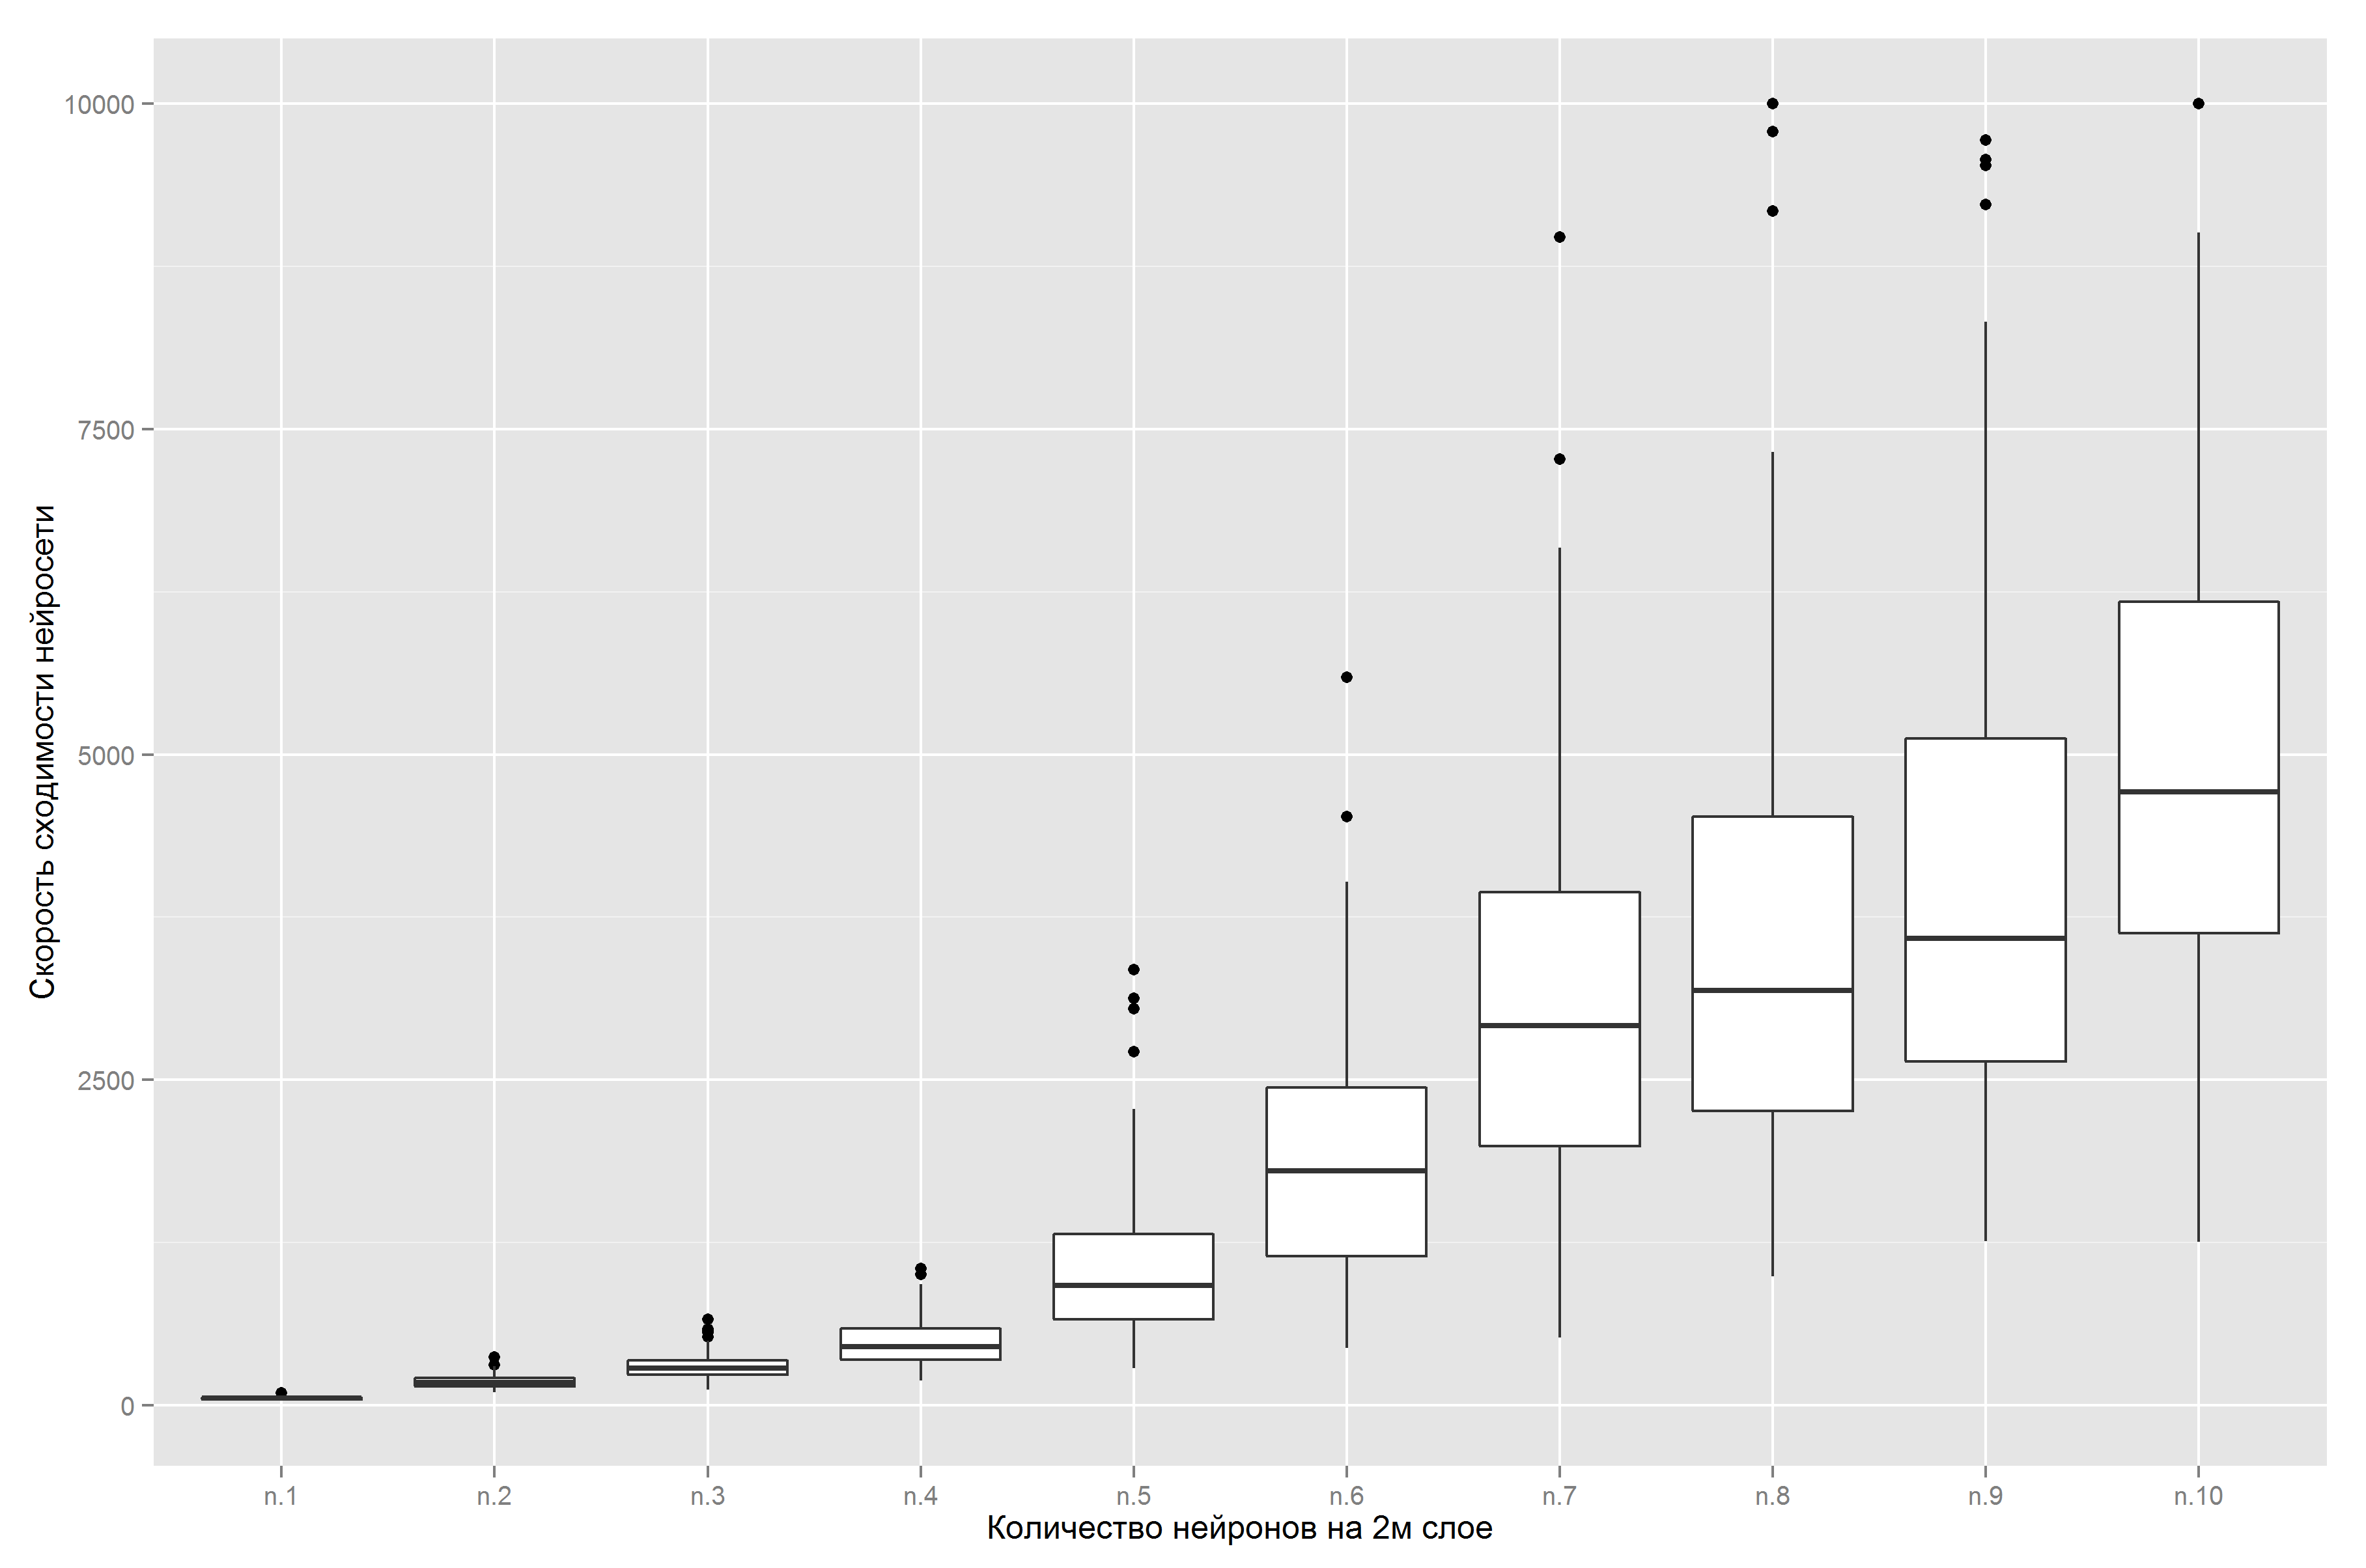
\includegraphics[width=10cm, height=7cm]{../../plots/n100L3_pn_vs_Tsync.png}

\end{center}
\end{frame}


\subsection{Оптимальное время синхронизации}
\begin{frame}
\frametitle{Оптимальное время синхронизации}
Каковы оптимальные параметры системы (N, L, кол-во нейронов на 1м слое) с точки зрения времени синхронизации и ключа?

\end{frame}


\subsection{Эффективность по ср. с другими способами обмена ключами}
\begin{frame}
\frametitle{Ср. с другими способами обмена ключами}
\begin{itemize}

\item Что будет если внедрить в TLS
\item Насколько велика экономия вычислительных операций и передач по сети по сравнению с Диффи-Хеллманом, задачей дискретного логарифмирования
\item Возможные применение
\end{itemize}

\end{frame}
\end{document}